
\documentclass[a4paper,letterpaper, 11pt, onecolumn]{article} %mettere 		                                    twoside se stampo fronte retro!!!
\usepackage[margin=0.9in]{geometry}
\usepackage[english]{babel}
\usepackage[T1]{fontenc}
\usepackage[latin1]{inputenc}
\usepackage{graphicx}
\usepackage{subfigure}
\usepackage{amsmath}					%formule matematiche
\usepackage{amssymb}	
\usepackage{titling}


\begin{document}

\title{People Detection \\with Histogram of Oriented Gradients \\
\large Project report}
\author{Chiara Bizzotto, Maurizio Ingrassia and Roberta Papa}

\maketitle

\begin{abstract}
In this report we present a possible method for human detection in videos. We implemented an algorithm in Python that uses Histograms of Oriented Gradient descriptors, associated with Support Vector Machine (SVM) classifier with linear kernel, for detecting people in scene. A sliding window checks through a binary mask if there is movement in that region of interest avoiding in this way unnecessary checks and wrong detections. The features extracted from those rectangular regions with movement are thus processed from the SVM which decides if it contains a person or not.
Finally we evaluated the efficiency of our method both in the preliminary single-scale case and in the multiscale one, added to get over some of the constraints.
%The method proposed works with a single scale, using the distance between the corners of the detection and the ground-truth. Later, a second approach has been used trying to get over the limits of the first method using a multiscale analysis with a region overlapping evaluation.
\end{abstract}

\section{Introduction}
Detecting human beings in a given scene represents one of the most important and challenging tasks in computer vision and is becoming a key technology for many areas.
Our project aims to apply one of the techniques used in literature, based on Histogram of Oriented Gradients (HOG), to detect people in a scene. 

The minimum target of our work is that each person must be found at least once in a set of frames: in this way our algorithm could be easily used, after some improvements, in a video-surveillance system.

Our project has some constraints, due to the choices taken during the set-up of the work, that make it suitable for specific contexts only: the detection is limited to moving pedestrians, i.e. our algorithm can find only people walking and not people standing still. Furthermore, to make the choice of parameters easier, we have decided to limit our range of action to fixed-camera videos and to use only one scale for the detection.

Section \ref{dataset} describes the Data-sets chosen for the experiment both for the Training and for the Validation/Test of the model. Section \ref{algorithm} explains in details the additions we have implemented to the standard algorithm (HOG descriptor and SVM classifier). Section \ref{results} presents the numerical results obtained applying our algorithm to the data-set and finally in Section \ref{discussion} we discuss the results obtained and we propose some improvements to the method.


\section{The Data-set}\label{dataset}
The data-set used for the training is composed, for the positive example, of the \emph{ViPeR Data-set} and for the negative examples of a custom-made one (see Figures \ref{fig:dataset} a-e), where one can find background, objects and ``pieces'' of people. 
The size of the images is 48x128 pixels which we treat as the base dimension for the window (Section \ref{algorithm}). In total we used more than 6000 images for the training.

For the validation and the training we took a set of videos from \emph{3dPes} (for example Figure \ref{fig:dataset} f) of about 200 frames each on average where from 1 to 10 persons walk in the scene. One of the major obstacles of this data-set is the difficult light condition.

Data-set annotations have been done manually for the whole set, which leads sometimes to a little misalignment with the region detected: this affects the evaluation of the performance both in positive and in negative, thus we think that the total effect can be neglected.
\\
\begin{figure}[h!]
\centering
\subfigure[]{
\includegraphics[height=3cm]{000_45.PNG} }
\subfigure[]{
\includegraphics[height=3cm]{004_0.PNG} }
\subfigure[]{
\includegraphics[height=3cm]{009_45.PNG} }
\subfigure[]{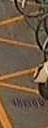
\includegraphics[height=3cm]{img_3300.JPG} }
\subfigure[]{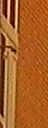
\includegraphics[height=3cm]{img_60040.JPG} }
\subfigure[]{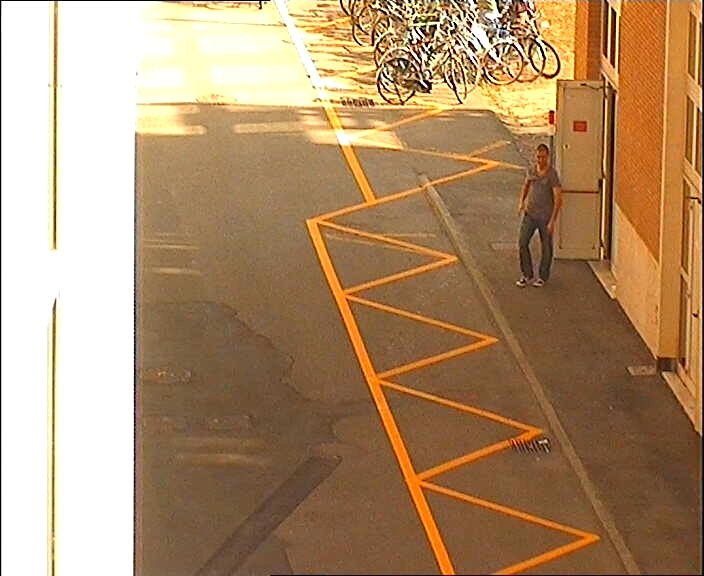
\includegraphics[height=3cm]{video0031.JPG} }

\caption{(a)-(c): Positive examples for training, (d)-(e): Negative examples for training, (f): Frame example for validation and test.}
\label{fig:dataset}
\end{figure}
\\



\section{The Algorithm}\label{algorithm}
\
\begin{figure}[h!]
\centering
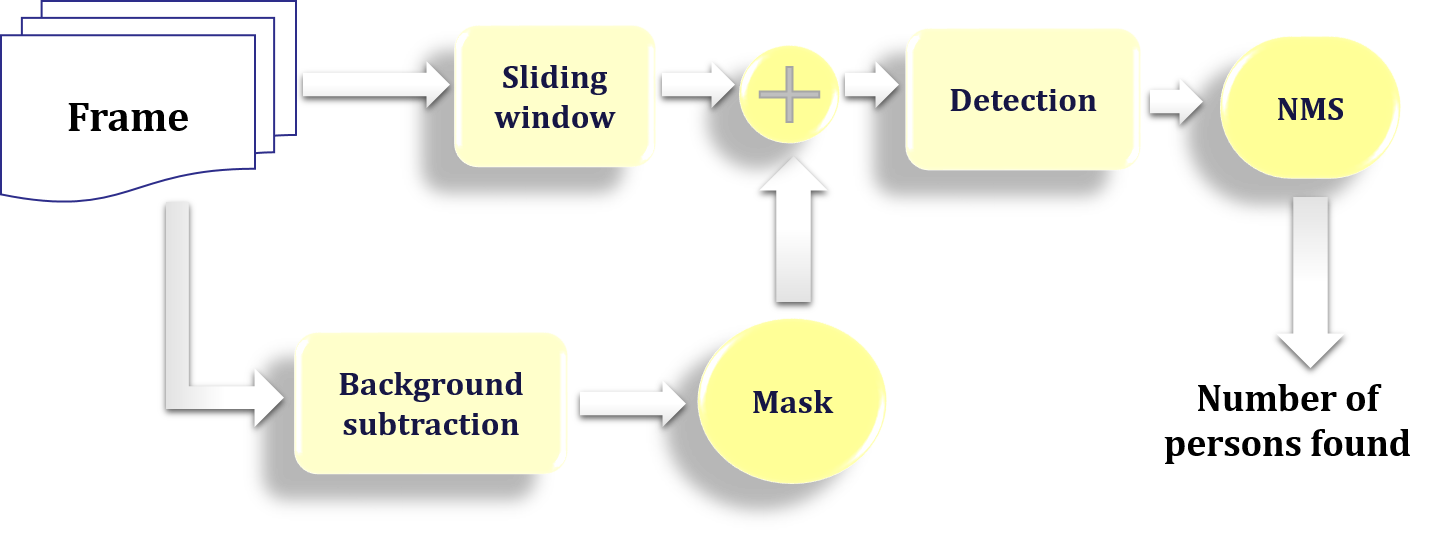
\includegraphics[width=0.9\textwidth]{schema.png} 
\caption{Block diagram of the algorithm}
\label{fig:diagram}
\end{figure}
\

The algorithm we implemented is briefly described in the block scheme in Figure \ref{fig:diagram}. For each frame of the video we extract the background using an iterative method that update the background $B$ as follows: 
\
$$B(t) = \alpha B(t-1) + (1-\alpha) I(t)$$
\
where $I(t)$ is the intensity (gray-scale) of the current frame and $\alpha$ is a weight that represents the trade-off between the relevance of the actual frame and the previous ones.
This allows us to build a mask that highlights only the regions of the frame in which there is movement. We tried two types of masks: one based on contrast (using gray-scale frames) and the other based on saturation (using HSV frames). For our application we combined the two masks by summing them, to obtain more robust regions (see Figure \ref{fig:mask}a). 
\begin{figure}[h!]
\centering
\subfigure[]{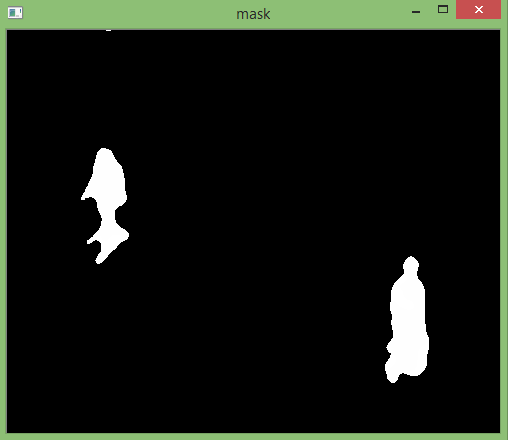
\includegraphics[height=4cm]{mask.png} }
\subfigure[]{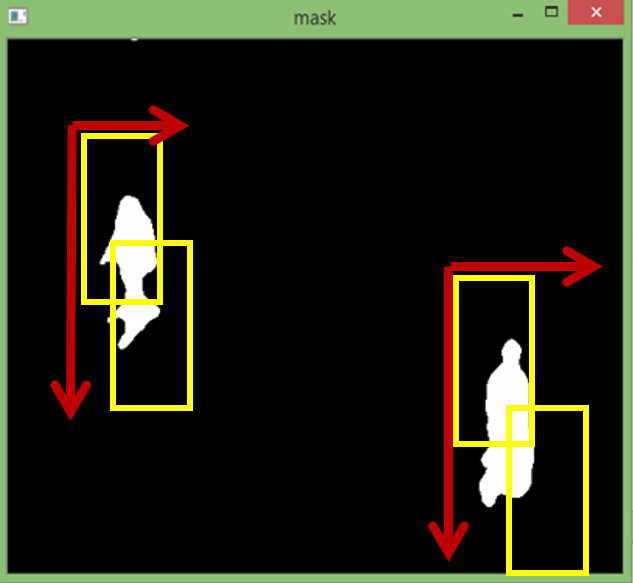
\includegraphics[height=4cm]{mask2.png} }
\caption{Example of mask with movement regions (a) and sliding window (b).}
\label{fig:mask}
\end{figure}

Once the mask has been calculated we perform the ``sliding window'' on the frame in exam (Figure \ref{fig:mask}b): a fixed-scale (with respect to the base one) window scans the frame and try for detection only if the number of white pixels, in the same ROI of the mask, is over a given threshold. For these windows we extract the feature vectors (HOG descriptor\footnote{HOG parameters: 8 orientations bins, 16x16 pixels per cell, 1x1 cells per block}) and we send them to the SVM classifier to get a prediction of the class they belong to: Person or Non Person. We use a probabilistic approach for the matching, which also allows us to discard multiple detections around the same ROI: we choose only those predictions that have the probability higher of a fixed threshold. For what concerns the classifier, we choose to use the linear kernel instead of the intersection one because of the less computational cost. At this point it is still possible to have multiple detections for a single person: for this reason we perform \emph{Non Maxima Suppression} by keeping, in the neighbourhood  of a detected person, only the bounding box with the higher probability.

Afterwards one improvement has been made to the algorithm and one of its most important limits has been overcome: we introduced the multiscale detection by cycling on the dimension of the sliding window. 

The results obtained from our detector and the variations due to the multiscale will be presented in Section \ref{results}.




\section{Experimental results}\label{results}
The performance of the classification were evaluated by cross-comparison between ground-truth and people found by our system. To check the correctness of the prediction we used two different methods, the first based on a threshold on the distance between the corners of the two bounding boxes, and the second on the overlapping of the two areas. Information on the goodness of our predictions were obtained computing Accuracy rate, Recall, Precision and F1-score derived from the confusion matrix as follows:
\\
$$Accuracy = \frac{TP + TN}{TP + TN + FP + FN}$$

$$Precision = \frac{TP}{TP + FP}$$

$$Recall = \frac{TP}{TP + FN}$$

$$F1-Score = \frac {2 TP}{2 TP + FP + FN}$$
\\
\begin{itemize}
\item False  positives  (FP):  examples  predicted  as  positive,
which are from the negative class.

\item False  negatives  (FN):  examples  predicted  as  negative,
whose true class is positive.

\item True positives (TP): examples correctly predicted as per-
taining to the positive class.

\item True negatives (TN): examples correctly predicted as be-
longing to the negative class
\end{itemize}

The  evaluation  measure  most  used  in  practice  is  the accuracy  rate. It  evaluates  the  effectiveness  of  the classifier by its percentage of correct predictions. The recall is the proportion of examples belonging to the positive  class  which  were  correctly  predicted  as  positive. Precision is a measure which estimates the probability that a positive prediction is correct and the F1-score is the harmonic mean of precision and recall.

In order to obtain the best performances these evaluation measures have been calculated changing the parameters of the model, in term of step of the sliding window, threshold of the mask and the C-value of the linear SVM (see Figures \ref{fig:step} and \ref{fig:cvalue}), for each video and then averaged them on the entire validation-set.

The first graph (Figure \ref{fig:step}) shows how the method performs worse by increasing the step of the sliding window, because it increases the chance of missing a person. We choose not to decrease the window stride under 11 because the computational costs were too high compared with the gain in detection accuracy. The matching threshold represents the probability we set as a threshold during the prediction in a specific ROI.
\begin{figure}[h!]
\centering
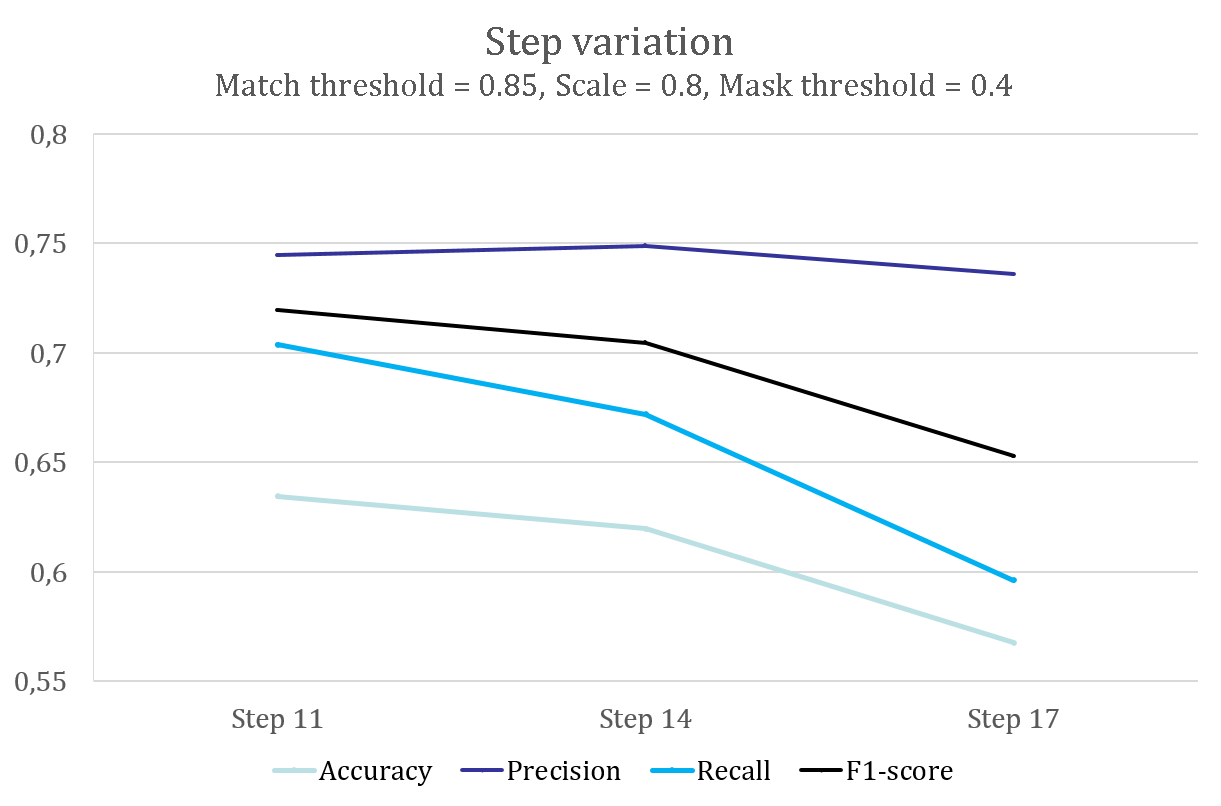
\includegraphics[height=6.5cm]{step_variation.png} 
\caption{Performances as the step of the sliding window change (single scale case).}
\label{fig:step}
\end{figure}

The second chart (Figure \ref{fig:cvalue}) show the consequences of the variation of the C-value with single-scale of the sliding window (a) and multiscale (b) related to the best parameters choosen by tuning them on the entire validation set. It is clear how the general performance of the algorithm, given by the F1-Score, does not change significantly from the first to the second case; on the contrary there is a slightly larger difference in terms of precision and recall (see Table \ref{tab:res}). In fact with multiscale the recall increases because, by looking for people of ``different sizes'', the algorithm has more possibilities of detecting a person; however on the other side, because of the low robustness of HOG descriptors,  the precision decreases: in our case this is not due to the increasing of the number of false positives but to an incorrect positioning of the detection window. 

\begin{figure}[h!]
\centering
\subfigure[]{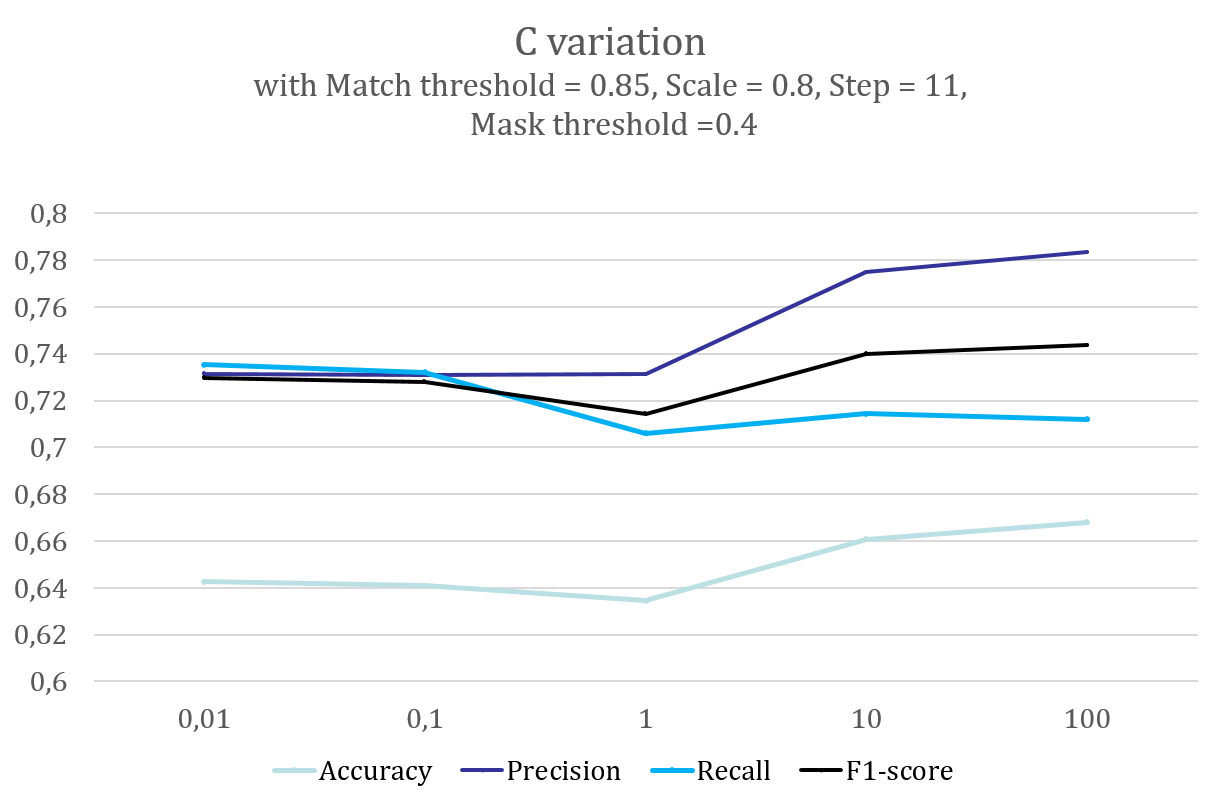
\includegraphics[width=0.7\textwidth]{c_variation.png} }\\
\subfigure[]{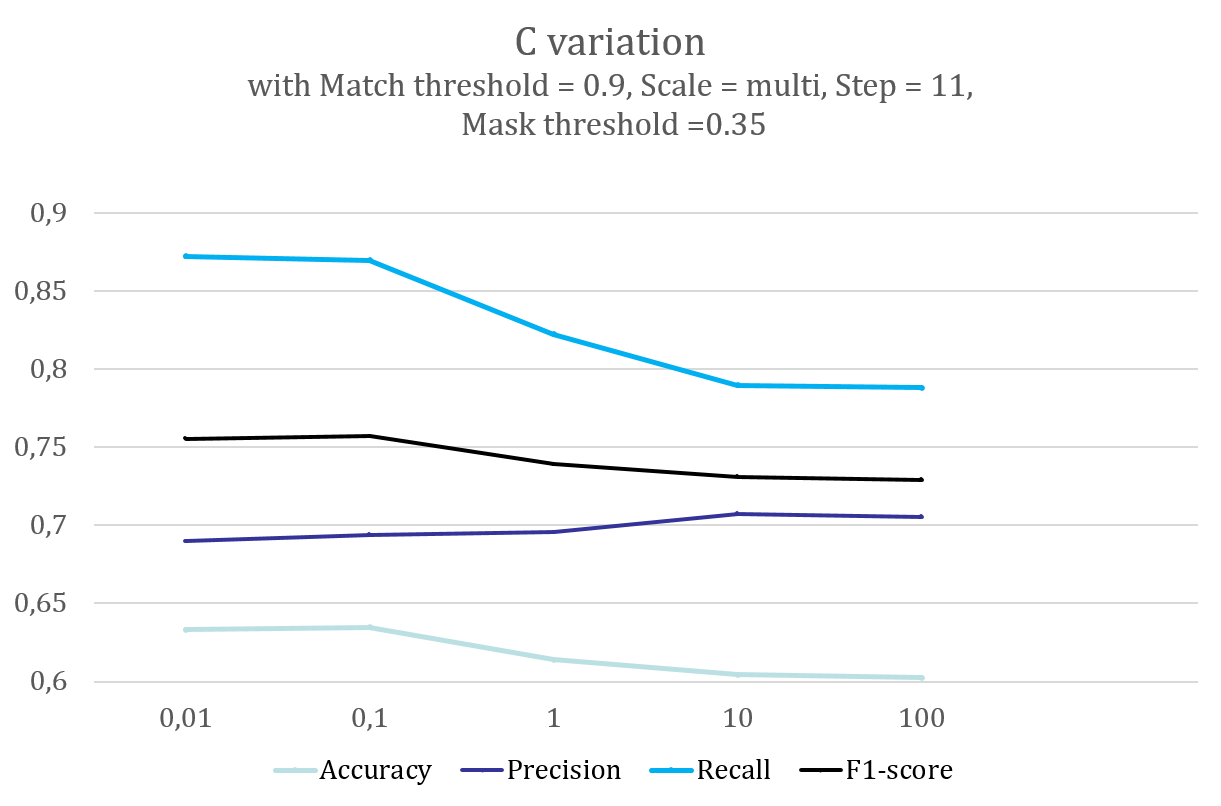
\includegraphics[width=0.7\textwidth]{c_variation_multi.png} }
\caption{Performances as the C-value changes in the single-scale case (a) and in the multiscale case (b) with best parameters for each algorithm.}
\label{fig:cvalue}
\end{figure}
\
\begin{table}[h!]
\centering
\begin{tabular}{c||c|c}
&\textbf{Fixed scale} & \textbf{Multiscale}\\
\hline \hline 
\textbf{Accuracy} &0.660 & 0.633\\
\textbf{Recall} &0.714  & 0.872\\
\textbf{Precision} & 0.775 & 0.690\\
\textbf{F1-score} & 0.740& 0.755\\
\end{tabular}
\caption{Final results with the best parameters of each algorithm: fixed scale = 0.8, step = 11 (for both algorithms), match threshold = 0.85 for single-scale and 0.9 for multiscale, mask threshold = 0.4 for single-scale and 0.35 for multiscale. }
\label{tab:res}
\end{table}

\section{Discussion}\label{discussion}
In this report we implemented a people detection algorithm: in particular we proposed two variations, one based on fixed scale detection and the other on multiscale, that is an improvement to the first solution. Despite the better results, the greater computational cost of the multiscale does not let the algorithm run real-time like the single-scale does. 
Interesting results are obtained using the multiscale in those videos where there is a grater number of people: with multiscale we can better manage the ``crowd'' achieving improvements in classification performances (see Table \ref{tab:performance compairson}).


Concerning future modifications, we can think of enhancing the dataset, in particular by adding more negatives examples. Moreover, we can introduce some kind of parallel computing to have a better response and work in real-time even with multiscale. 

Other possible future developments of our algorithm could be done applying Principal Component Analysis (PCA) to reduce the dimensionality of the feature vectors and testing different classifiers. Performing PCA could be also a good solution to decrease the computational cost of multiscale making it faster and letting the algorithm run real-time. Furthermore other kinds of descriptors could be tried because the HOG is not robust in case of occlusions or object with high variations with respect to the background.

%Another possibility could be to try with another kind of feature vectors, because the HOG descriptor is not robust in case of occlusions or object with high variations with respect to the background. Possible future developments to the algorithm could be done applying Principal Component Analysis (PCA)to reduce the dimensionality of the feature vectors and testing other classifiers. 
\
\begin{table}[h!]
\centering
\begin{tabular}{c||c|c}
&\textbf{Fixed scale} & \textbf{Multiscale}\\
\hline \hline 
\textbf{Accuracy} &0.504 & 0.610\\
\textbf{Recall} &0.665  & 0.776\\
\textbf{Precision} & 0.629 &  0.740\\
\textbf{F1-score} & 0.647& 0.758\\
\end{tabular}
\caption{Performance comparison between Fixed-scale = 0.8 and multiscale in a video with more people}
\label{tab:performance compairson}
\end{table}
\
Figure \ref{fig:algorithm detection} shows an example of how our algorithm works.

\begin{figure}[h!]
\centering
\subfigure[]{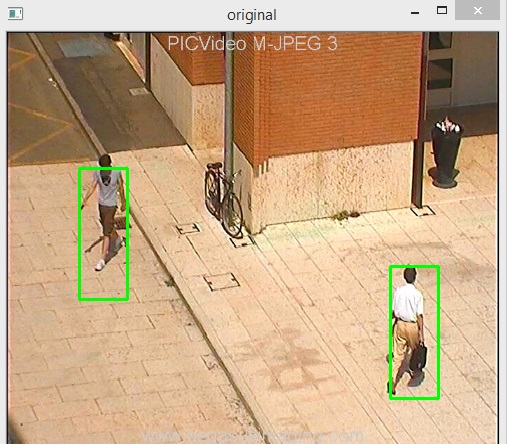
\includegraphics[height=10cm]{immagine1.JPG} }

\caption{Example of our algorithm detection.}
\label{fig:algorithm detection}
\end{figure}

\end{document}